% Chapter Template

\chapter{Methodology} % Main chapter title

\label{c4} % Change X to a consecutive number; for referencing this chapter elsewhere, use \ref{ChapterX}


\section{Data: }
The dataset in this study was collected from the Indian government portal CPCB. These datasets contain univariate Time series hourly data of 17 Indian cities,  with most cities providing approximately four years (see in \Cref{Eda1}). The table lists Bhiwadi,  Jodhpur,  Singrauli,  Ankleshwar,  Ludhiana,  Durgapur,  Yamuna Nagar,  Charkhi Dadri,  Jind,  Kurukshetra,  Sonipat,  Dharuhera,  Ambala,  Hisar,  Fatehabad,  Bulandshahr,  and Muzaffarnagar as the 17 cities from which data was collected shown on (\Cref{India map}) with Name,  Latitude and Longitude. The \Cref{Eda1} also provides information about the number of data points available in datasets, the highest number of data points in Jodhpur, and the lowest number of data points in Durgapur. In \Cref{Eda1}, All the datasets are thoroughly analysed based on several components such as Count, Min,  Mean,  Std,   25\%, Max,  75\%,  and 50\%. The detailed description of the analysis is then summarised for ease of understanding.




\begin{landscape}
    \setlength{\tabcolsep}{3pt}
  
    {\renewcommand{\arraystretch}{1}%
    \begin{longtable}[h!]{ p{0.06\linewidth} p{0.22\linewidth} p{0.12\linewidth} p{0.07\linewidth} p{0.06\linewidth}  p{0.06\linewidth} p{0.06\linewidth} p{0.06\linewidth} p{0.06\linewidth} p{0.06\linewidth} p{0.06\linewidth}}%{|l|l|l|l|l|l|}{llllllll}
    \caption{Statistical exploratory data analyses $($EDA$)$ of 17 Time Series Datasets of polluted Indian cities based on $PM_{2.5}$ \cite{bhawan2020central}.}
    \label{Eda1}\\
    \hline D.No. & DataSets & Year  & Samples &Mean &Std & Min &25\% &50\% &75\% & Max\\ \hline
    \endhead
    %
    \hline
    \endfoot
    %
    \endlastfoot
    %
    D1 &  BHIWADI          & 2017-2022  & 43394   & 108.03 & 79.76  & 0.02 & 55.22   & 97.32       & 135.36 & 999.99 \\ 
    D2 &  JODHPUR     & 2015-2022 &\textbf{61409} & 84.31 & 56.18 & 0.18 & 53.25   & 84.31 & 93.42   & 999.99 \\
    D3 &  SINGRAULI    & 2017-2022 & 43695   & 84.08 & 78.33 & 0.25 & 32.25   & 66          & 111.25  & 985    \\
    D4 &  ANKLESHWAR   & 2019-2022  & 33535     & 58.47 & 35.83 & 0.51 & 32.75   & 58.47 & 72.24   & 977.39 \\ 
    D5 &  LUDHIANA        & 2017-2022  & 49010  & 54.18 & 41.73 & 0.07 & 29.7    & 47.66       & 64.88   & 999.99 \\
    D6 &  DURGAPUR       & 2020-2022 & \textbf{17434}   & 71.67 & 46.20 & 0.33 & 37.47 & 62.05      & 98.03 & 565.41 \\ 
    D7 &  YAMUNA\_NAGAR  & 2019-2022 & 34299   & 77.86  & 52.31 & 0.1  & 43.8    & 69.91       & 94.28   & 930    \\
    D8 &  CHARKHI\_DADRI  & 2020-2022  & 24099   & 80.19 & 62.81 & 0.01 & 39.54  & 77.92       & 94.49  & 995.1  \\ 
    D9 &  JIND             & 2019-2022 & 34145 & 81.21 & 71.20 & 0.2  & 38.99   & 61.45       & 98.25   & 845.6  \\ 
    D10 &  KURUKSHETRA    & 2019-2022  & 34208 & 68.75& 53.80 & 0.46 & 33.33   & 56.38       & 87.56   & 962.7  \\ 
    D11 &  SONIPAT        & 2019-2022  & 34362  & 54.88 & 43.21  & 0.02 & 27.87   & 49.4        & 62.72   & 543.1  \\ 
    D12 &  DHARUHERA     & 2019-2022 & 34265 & 78.86 & 59.21 & 0.02 & 40.9    & 70.32       & 92.85   & 838.9  \\
    D13 &  AMBALA         & 2019-2022 & 34174 & 61.58 & 45.39 & 0.02 & 32.94   & 51.27       & 76.18 & 754.89 \\
    D14 &  HISAR          & 2019-2022 & 34143 & 86.22 & 71.02 & 0.63 & 42.62   & 69.33       & 102.89 & 999.99 \\ 
    D15 &  FATEHABAD      & 2019-2022 & 34160 & 63.01 & 60.46 & 0.07 & 32.63   & 49.01       & 72.5    & 999.99 \\
    D16 &  BULANDSHAHR  & 2018-2022 & 39869  & 90.53 & 85.08 & 0.25 & 34      & 63.75       & 120.25  & 985    \\ 
    D17 &  MUZAFFARNAGAR  & 2018-2022 & 38786 & 89.29 & 72.84  & 1    & 42.75   & 81.25       & 102.25  & 986    \\ \hline
    \end{longtable}}
    \end{landscape}








  

% Figure
\begin{figure}[H]
	\centering
		\includegraphics[scale=0.32]{india_map}
	  \caption{Geographical representation of polluted cities of India with their Latitude,  Longitude and Name.}
    \label{India map}
\end{figure}


\begin{itemize}
\item \textbf{Preproccessing: }Data preprocessing is critical in the ML process as it ensures the data is clean,  consistent,  and ready for analysis. Techniques like missing value imputation and min-max scaling facilitate data normalisation and improve the effectiveness of machine learning algorithms by allowing them to learn from the data and make accurate predictions.
During the initial data preprocessing stage,  missing values are replaced with the means. The dataset is divided into ten parts or chunks,  and the mean is calculated for each chunk. Subsequently,  the means of all the chunks are averaged together,  as shown in \Cref{equ: mean}:
\begin{equation} \label{equ: mean}
        x_i=\frac{\sum_{i=1}^{k} \left(\frac{D_{c_{i}}}{D_{s_{i}}} \right)}{k}
\end{equation}
 where $k=10$ \& $x_i$ is missing value in time series and $D_c$ represent chanks of Dataset. $D_s$ is the number of available samples in the dataset chunks represented by $D_c$. \\
Once the missing values have been attributed in the dataset using \Cref{equ: mean}, the next step is to apply min-max scaling \Cref{equ: minmax}. This technique ensures that univariate data is scaled to fall within the range of [0, 1]. The scaling is achieved \Cref{equ: minmax}: 
\begin{equation}
        x_{norm,  i}=\frac{x_i - \mu}{max(x)-min(x)}
        \label{equ: minmax}
    \end{equation}
Where $x_i$ is the $i^{th}$ data point and $\mu$ is the mean of univariate data $min(x)$  and $max(x)$ denote the minimum values and maximum values in the univariate series. Consistency is essential for comparing data across different datasets. Additionally,  the scaling technique reduces the influence of outliers and enhances the data's robustness.
\item
\textbf{Decomposition and analysis: }
In \Cref{eda1,eda2,eda3}, all subplot has been plotted on 480 recent data points. \Cref{eda1,eda2,eda3} presents the graphical representation of the dataset,  showcasing different categories like trend \&  seasonal. In rows 1,  and 4  the data is labelled as "Original." Rows 2,  and 5 correspond to the "Seasonal" category,  while rows 3,  and 6 represent the "Trend" category. The last two row combines all three categories,  displaying "Original, " "Seasonal, " and "Trend" data in a single dataset. Each subplot within the graph has a specific dataset name,  indicated in the legend.
\par The graph consists of three columns,  each corresponding to a specific range of rows (1 to 3, and 3 to 6 ) from the dataset. The border colour remains consistent across these columns,  indicating they belong to the same dataset. The legend provides clarity by associating the dataset name with its respective subplot,  facilitating a comprehensive understanding of the data distribution and categories.


\begin{figure*}
  \centering
  \includegraphics[scale=0.3]{eda1}
  \caption{Decomposition of 17 data sets based on trend, seasonal, and original dataset.}
  \label{eda1}
\end{figure*}


\begin{figure*}
  \centering
  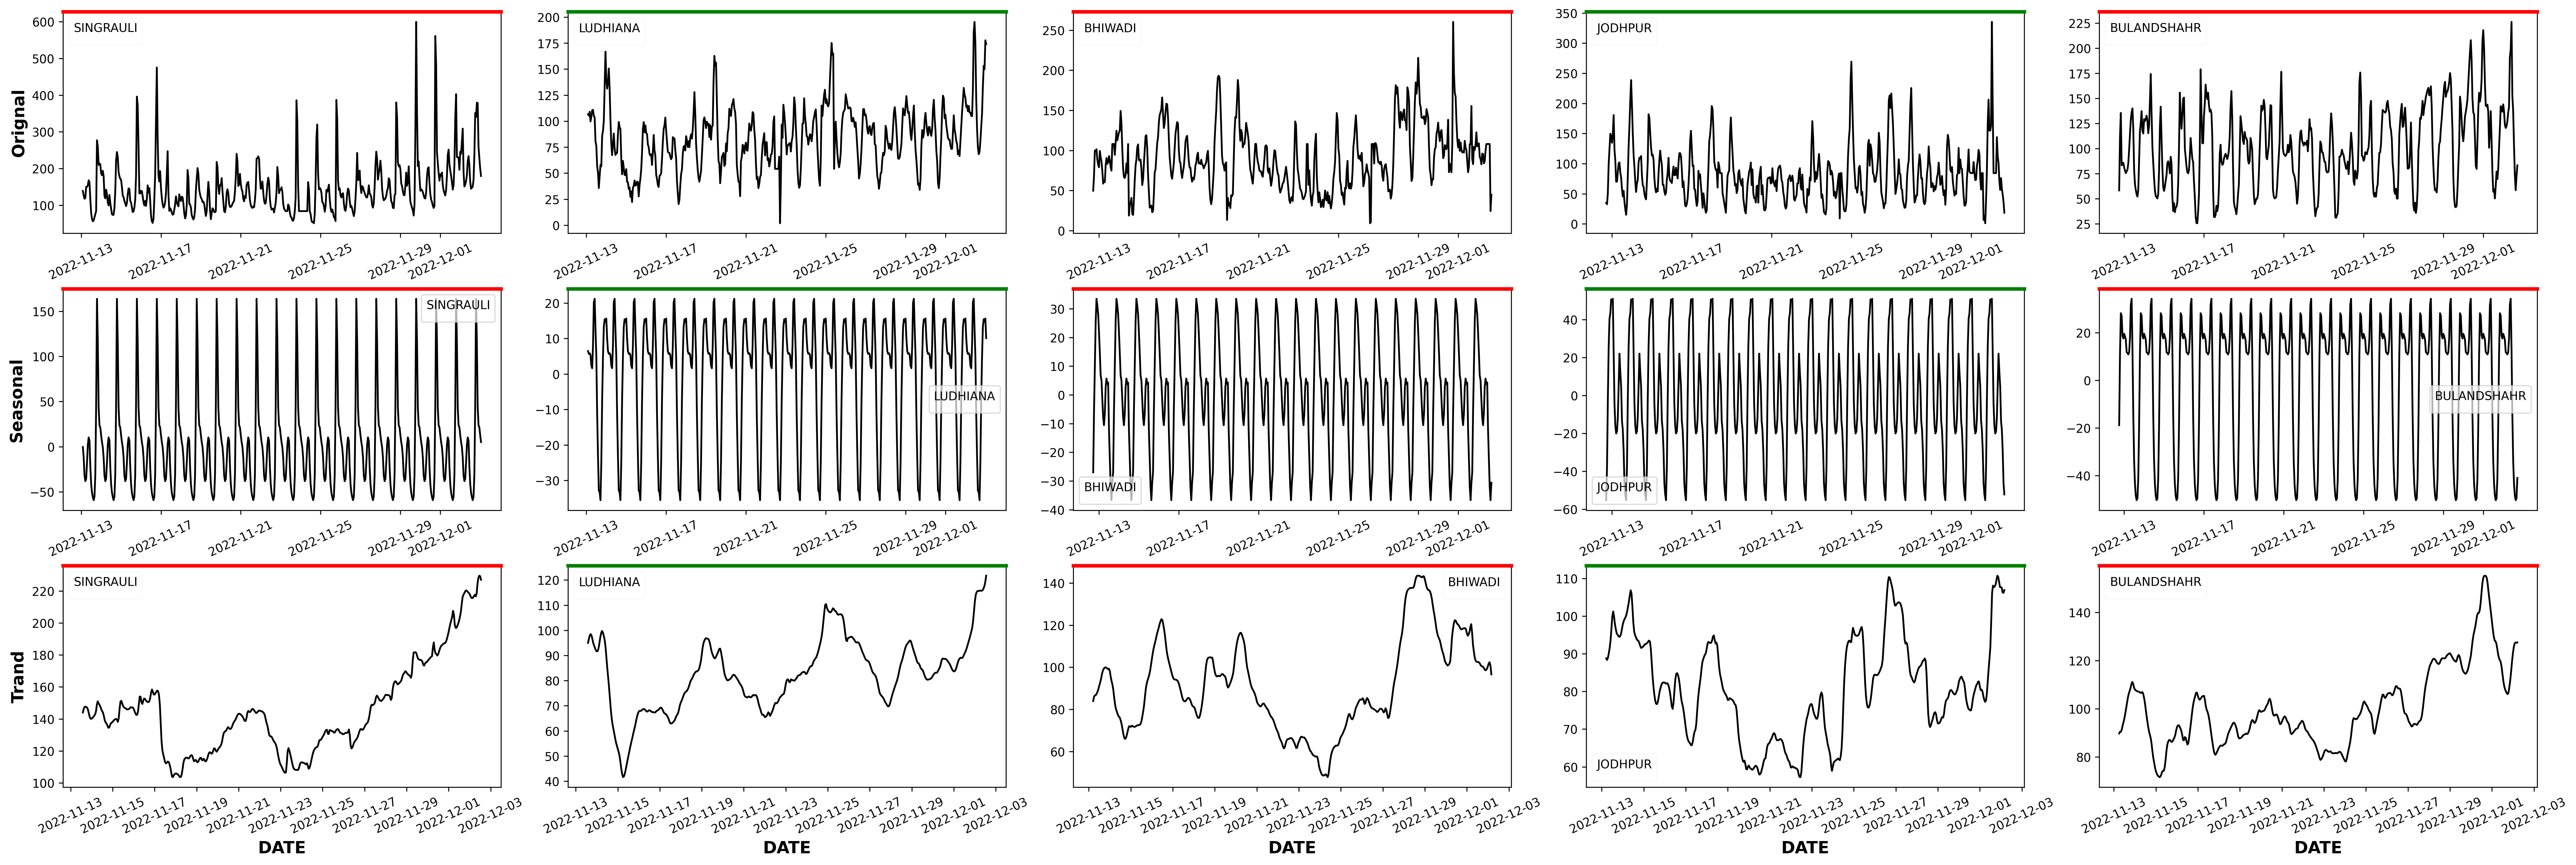
\includegraphics[scale=0.3]{eda2}
  \caption{Continuation of decomposition of 17 data sets based on trend, seasonal, and original dataset.}
  \label{eda2}
\end{figure*}


\begin{figure*}
  \centering
  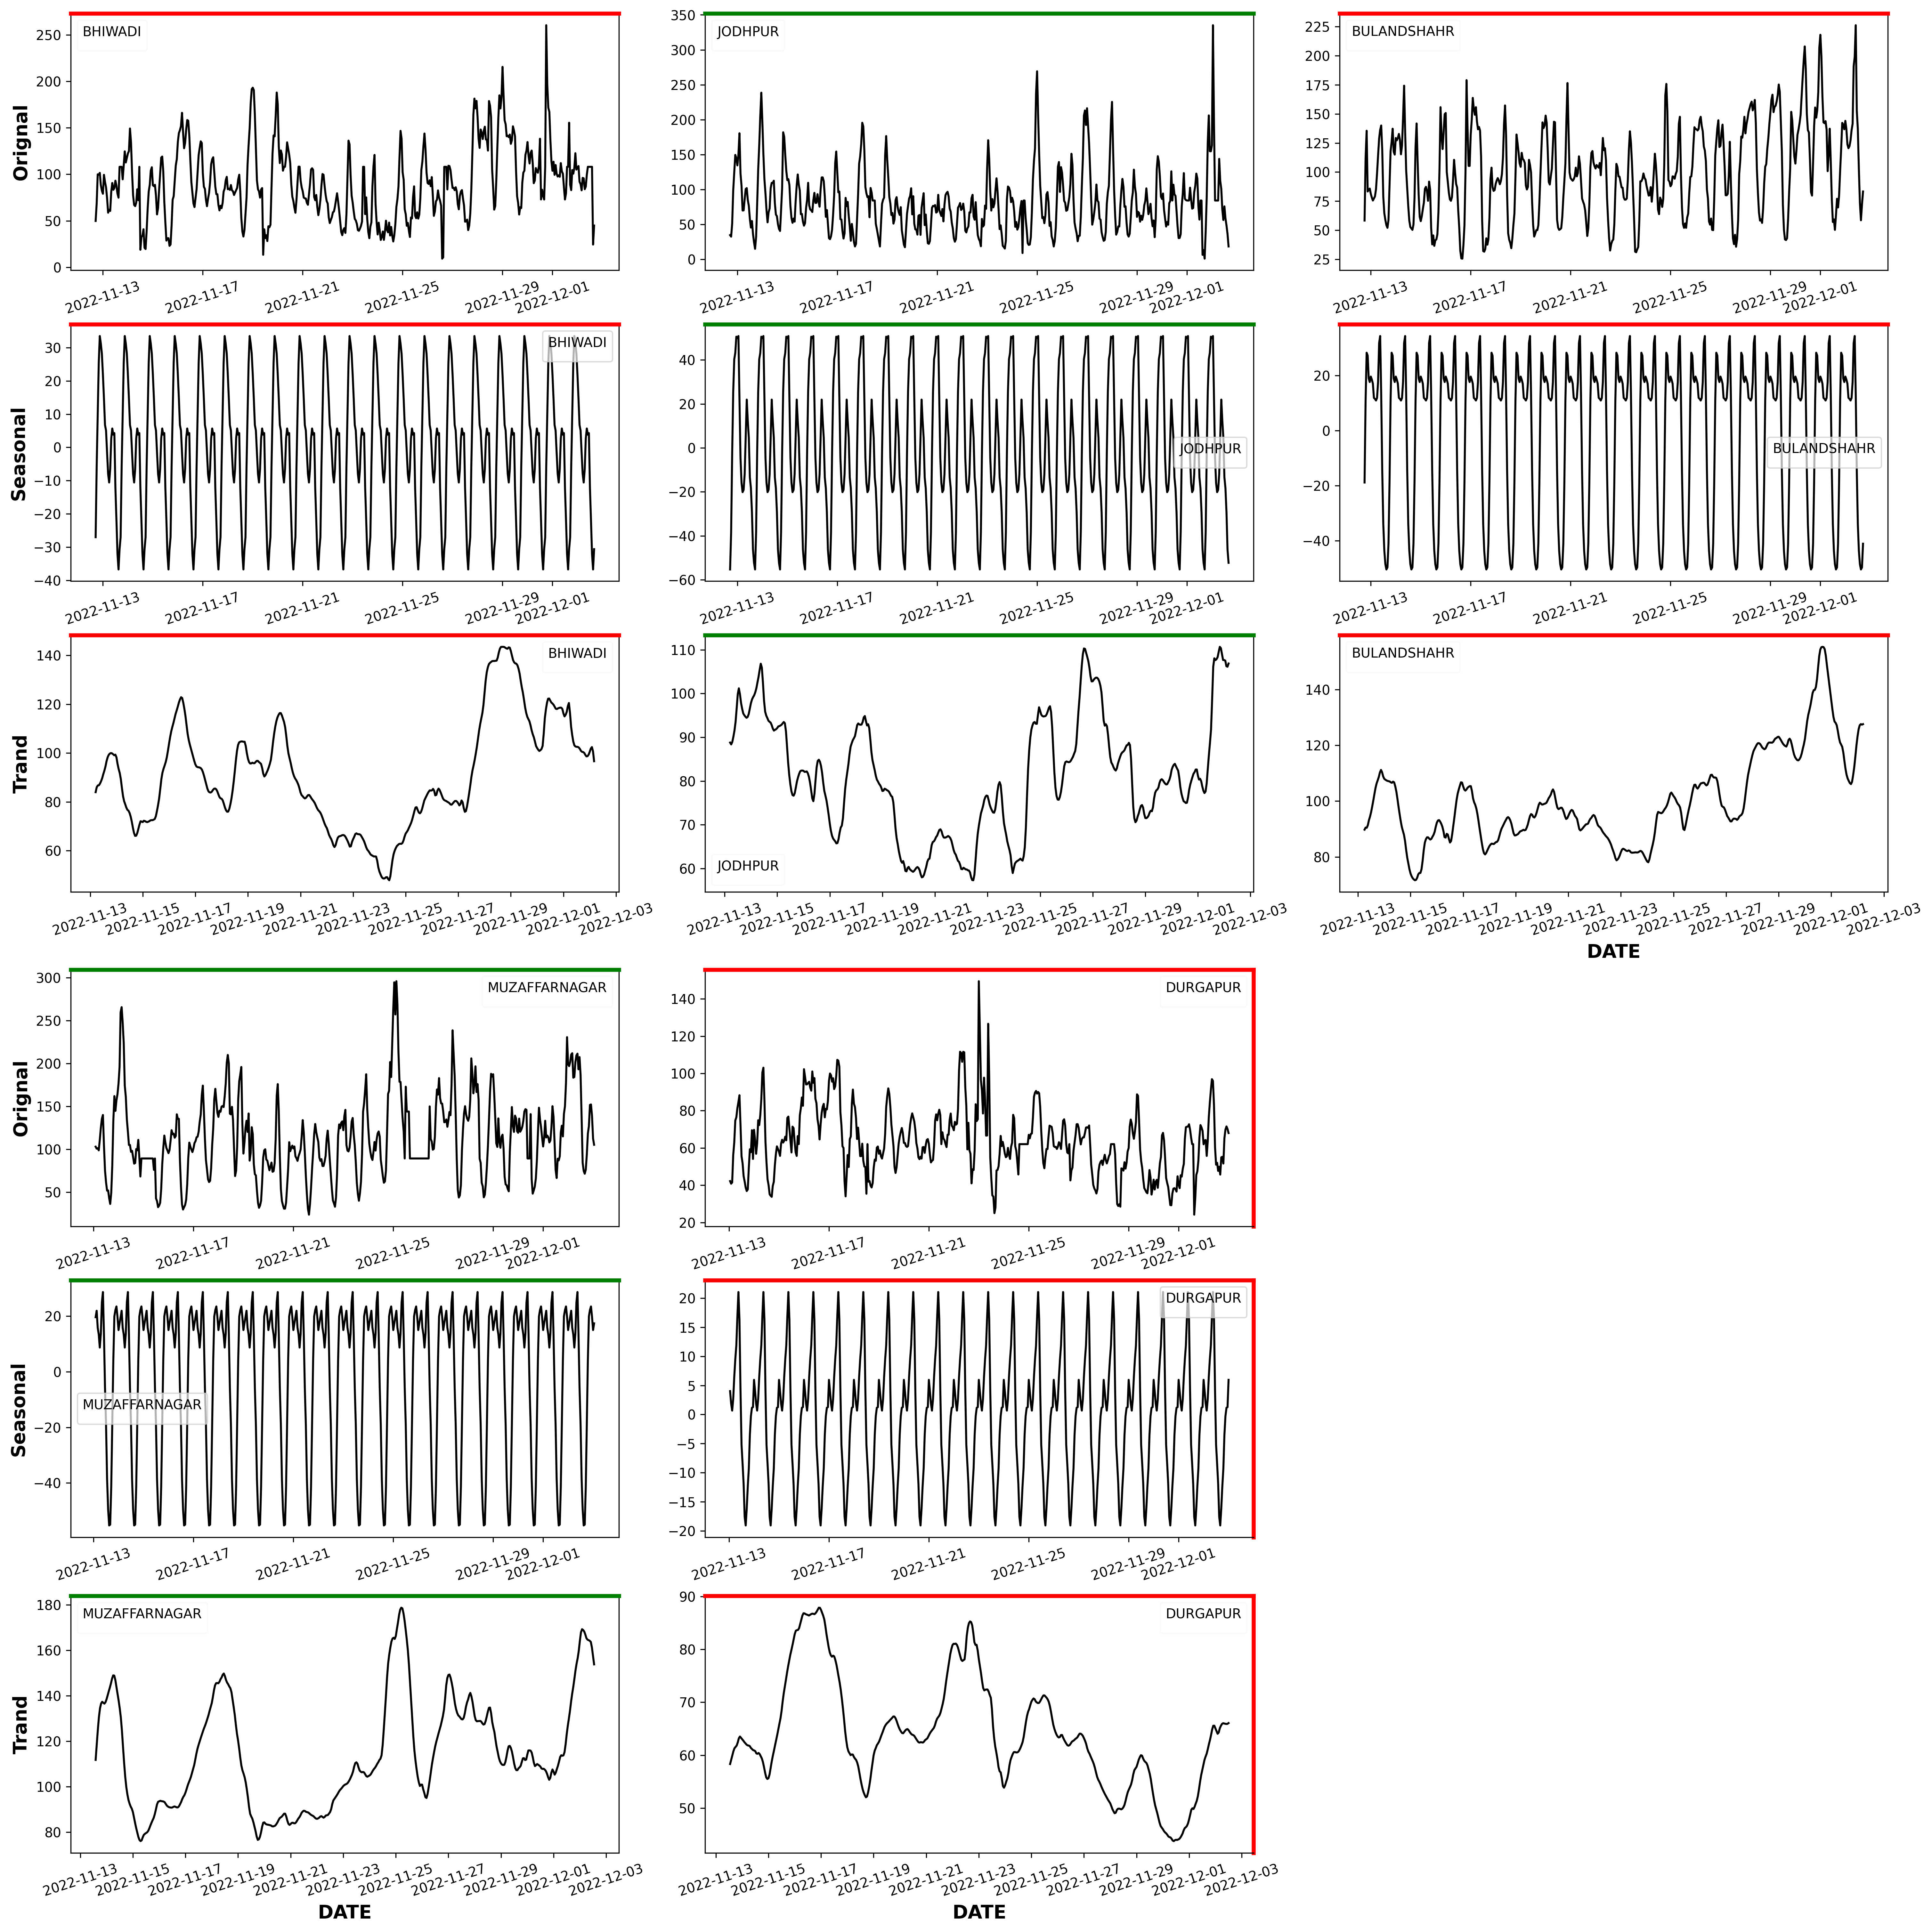
\includegraphics[scale=0.3]{eda3}
  \caption{Continuation of decomposition of 17 data sets based on trend, seasonal, and original dataset.}
  \label{eda3}
\end{figure*}



% \begin{figure*}[h!]
%   \centering
%   \subfigure{\includegraphics[scale=0.208]{eda1}}
%   \subfigure{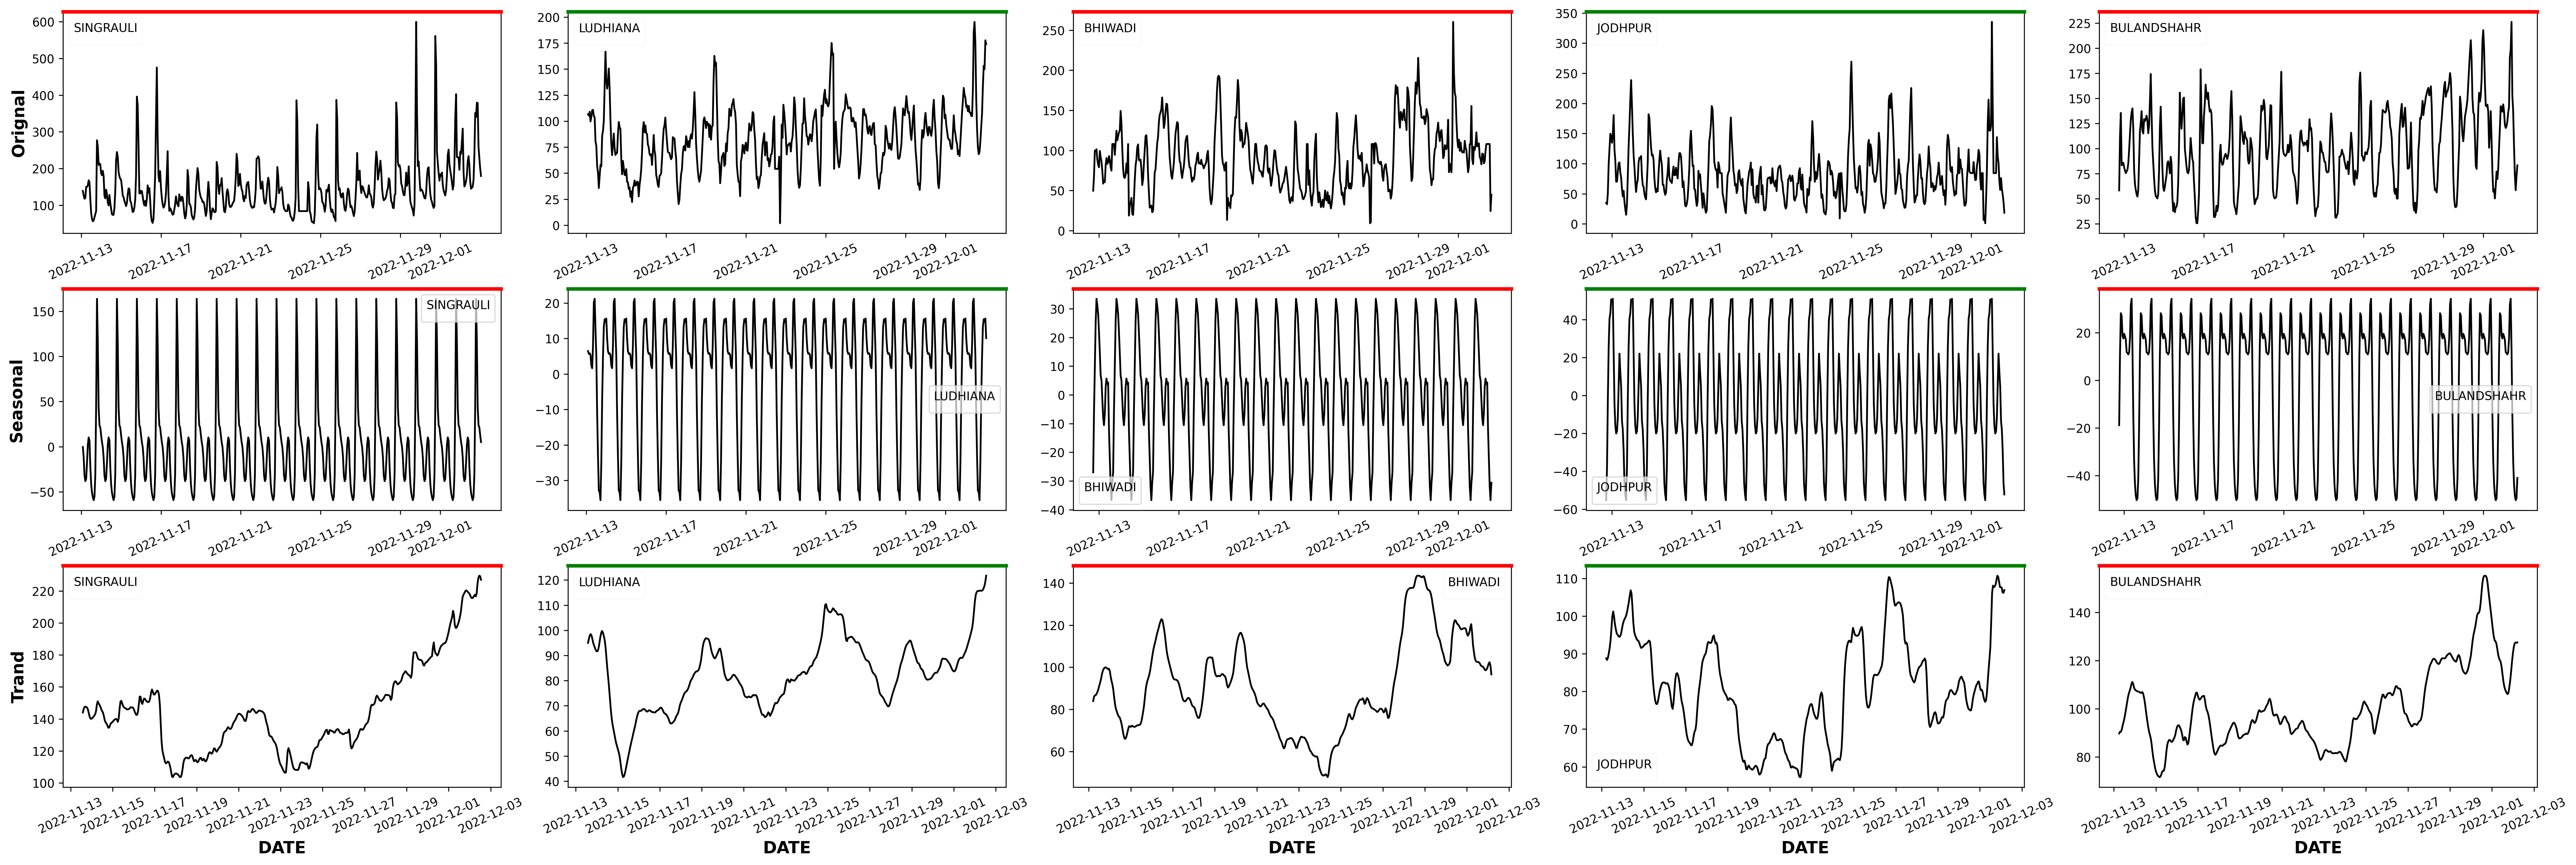
\includegraphics[scale=0.208]{eda2}}
%   \subfigure{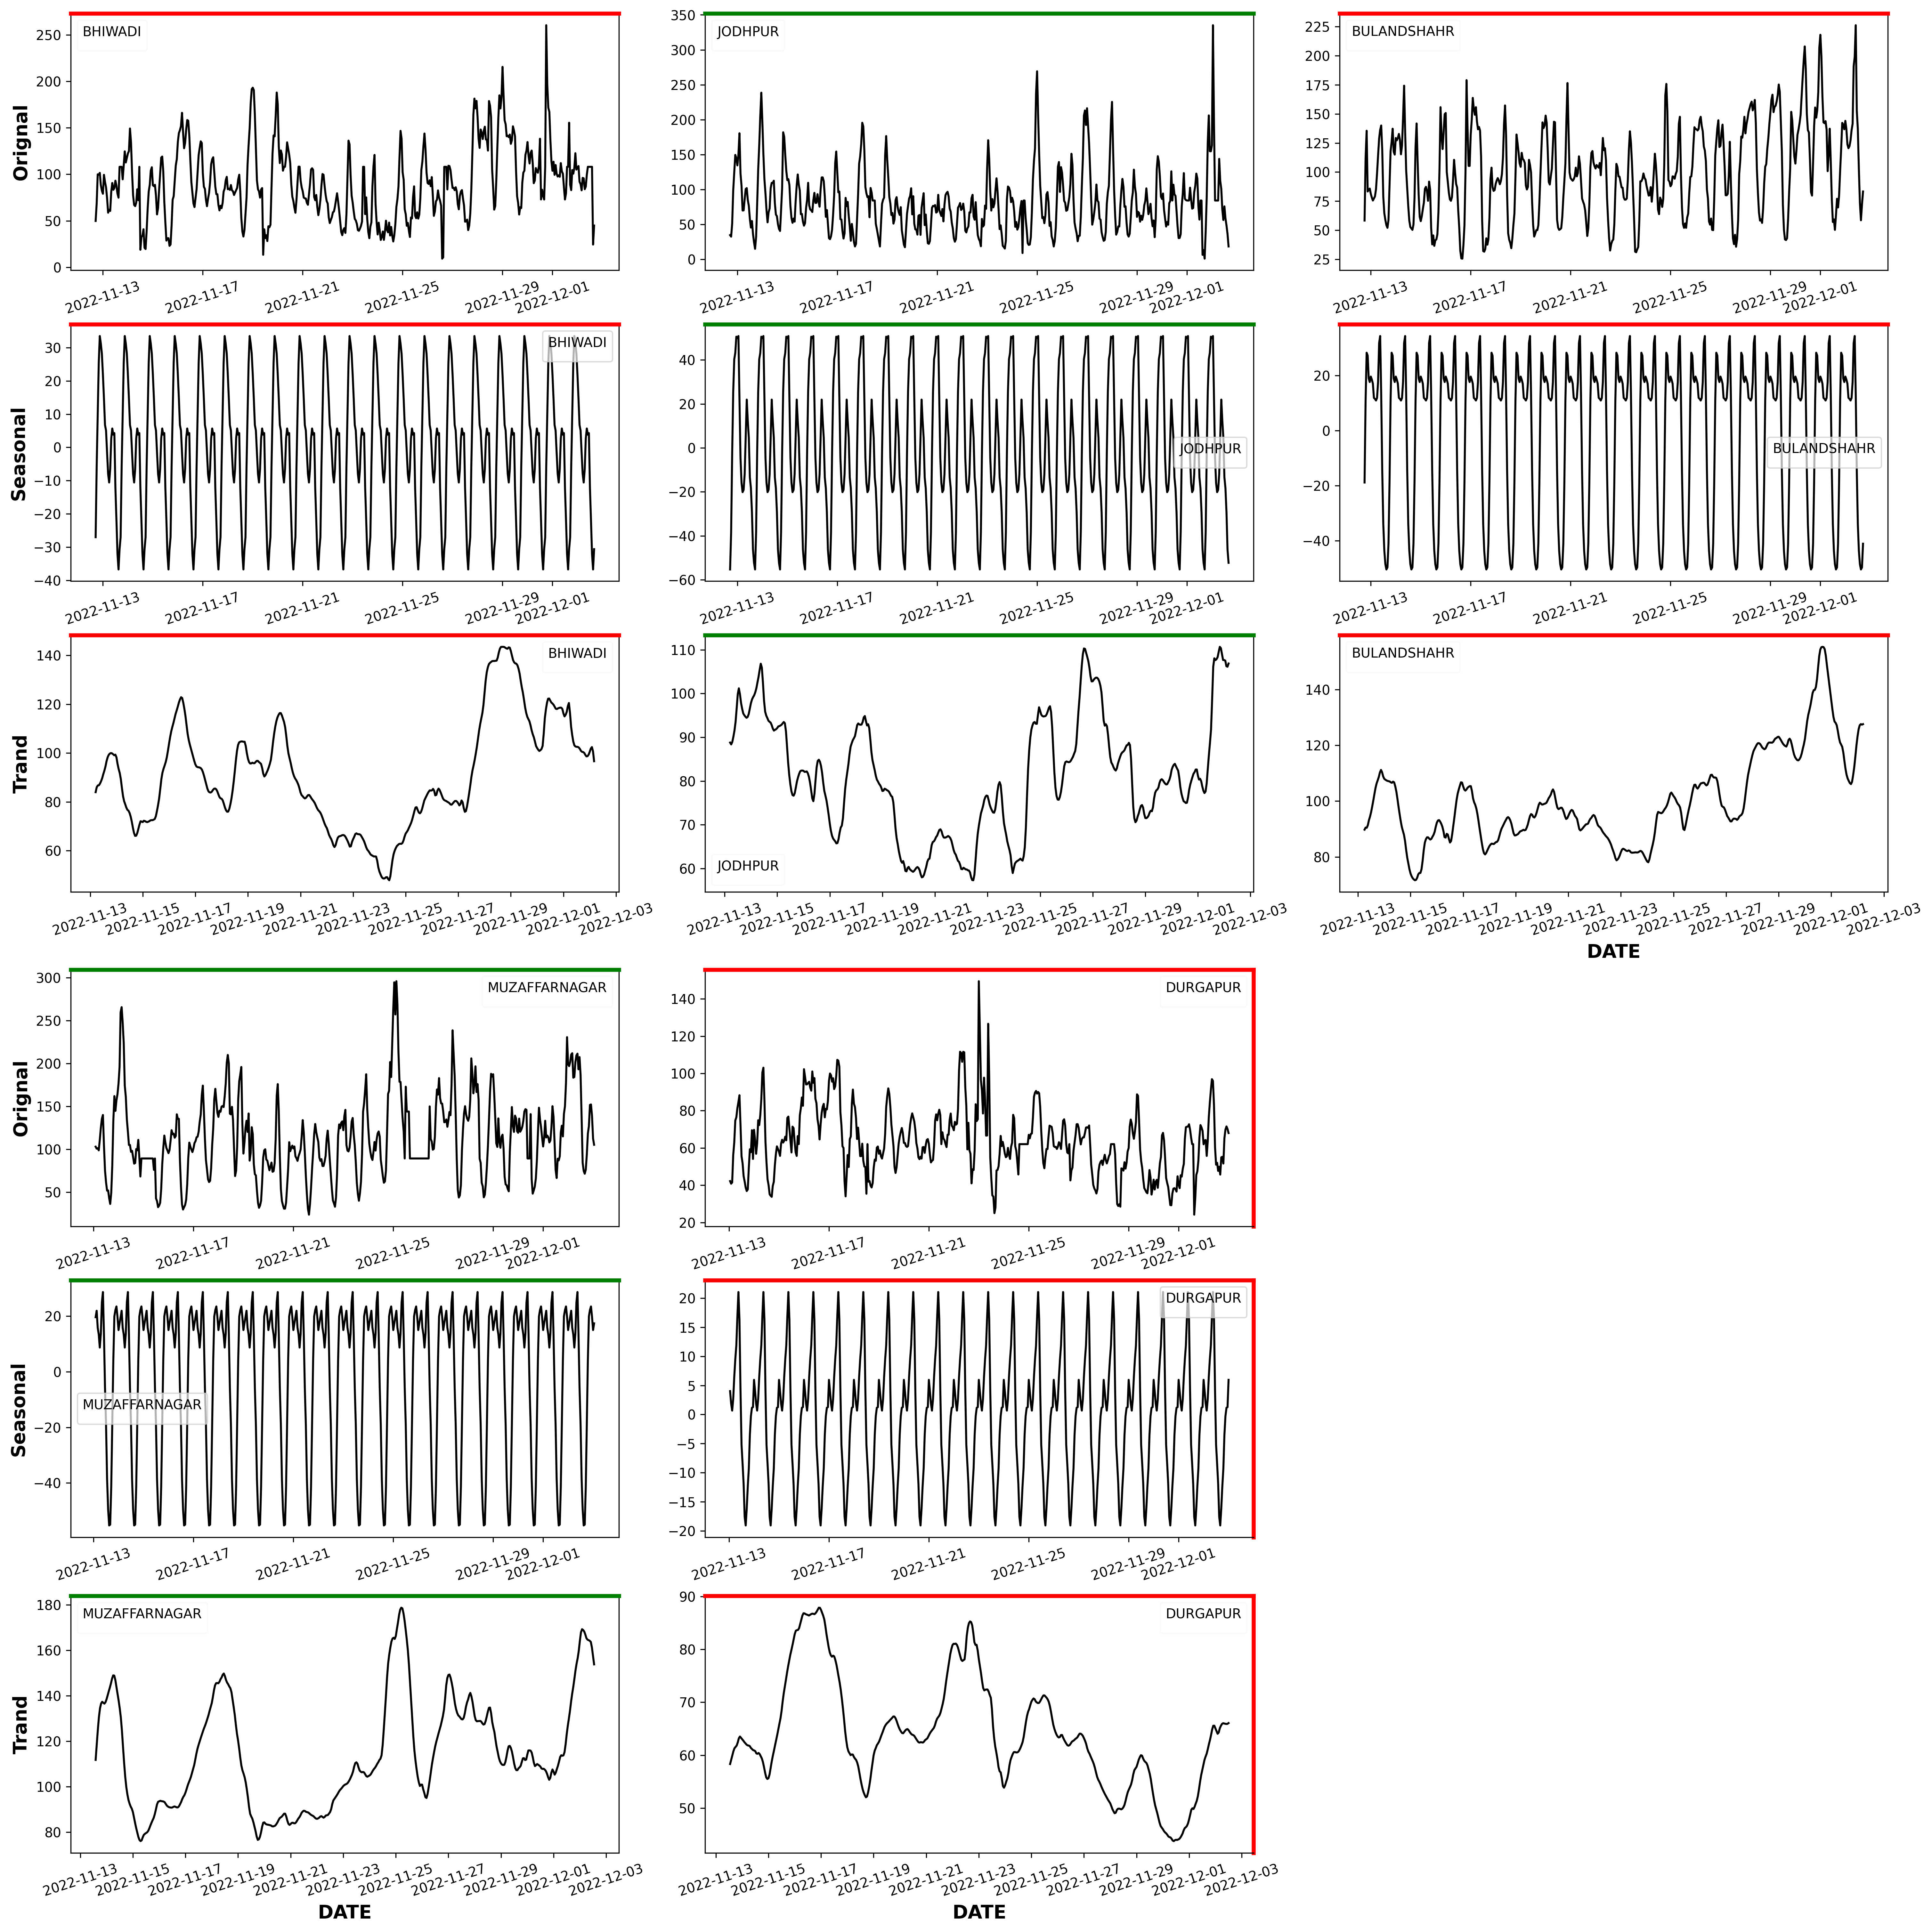
\includegraphics[scale=0.208]{eda3}}
%   \caption{Decomposition of 17 data sets based on trend, seasonal, and original dataset.}
%   \label{Eda}
% \end{figure*}

\par \Cref{eda1,eda2,eda3} illustrates the seasonal variations in the dataset with a frequency of every 24 hours. Each subplot within the graph contains 20 data points representing the seasonal pattern. Additionally,  the graph showcases various types of trends present in the data. These trends may include upward, downward,  or fluctuating trends over time. The combination of seasonal variations and diverse trends provides valuable insights into the underlying patterns and behaviours of the dataset.
\end{itemize}

\section{Method}
This research section will delve into the methodology of predicting $PM_{2.5}$ using various deep-learning models. Our data was obtained from the  CPCB (Central Pollution Control Board), India \cite{bhawan2020central} hourly univariate data collection. It focused on a single future $PM_{2.5}$ in this dataset. Then we processed the obtained data and implemented several deep-learning models to generate our forecasts. The primary objective of employing these is to enhance the model's accuracy of our predictions. 
% Figure
\begin{figure*}[h!]
	\centering
		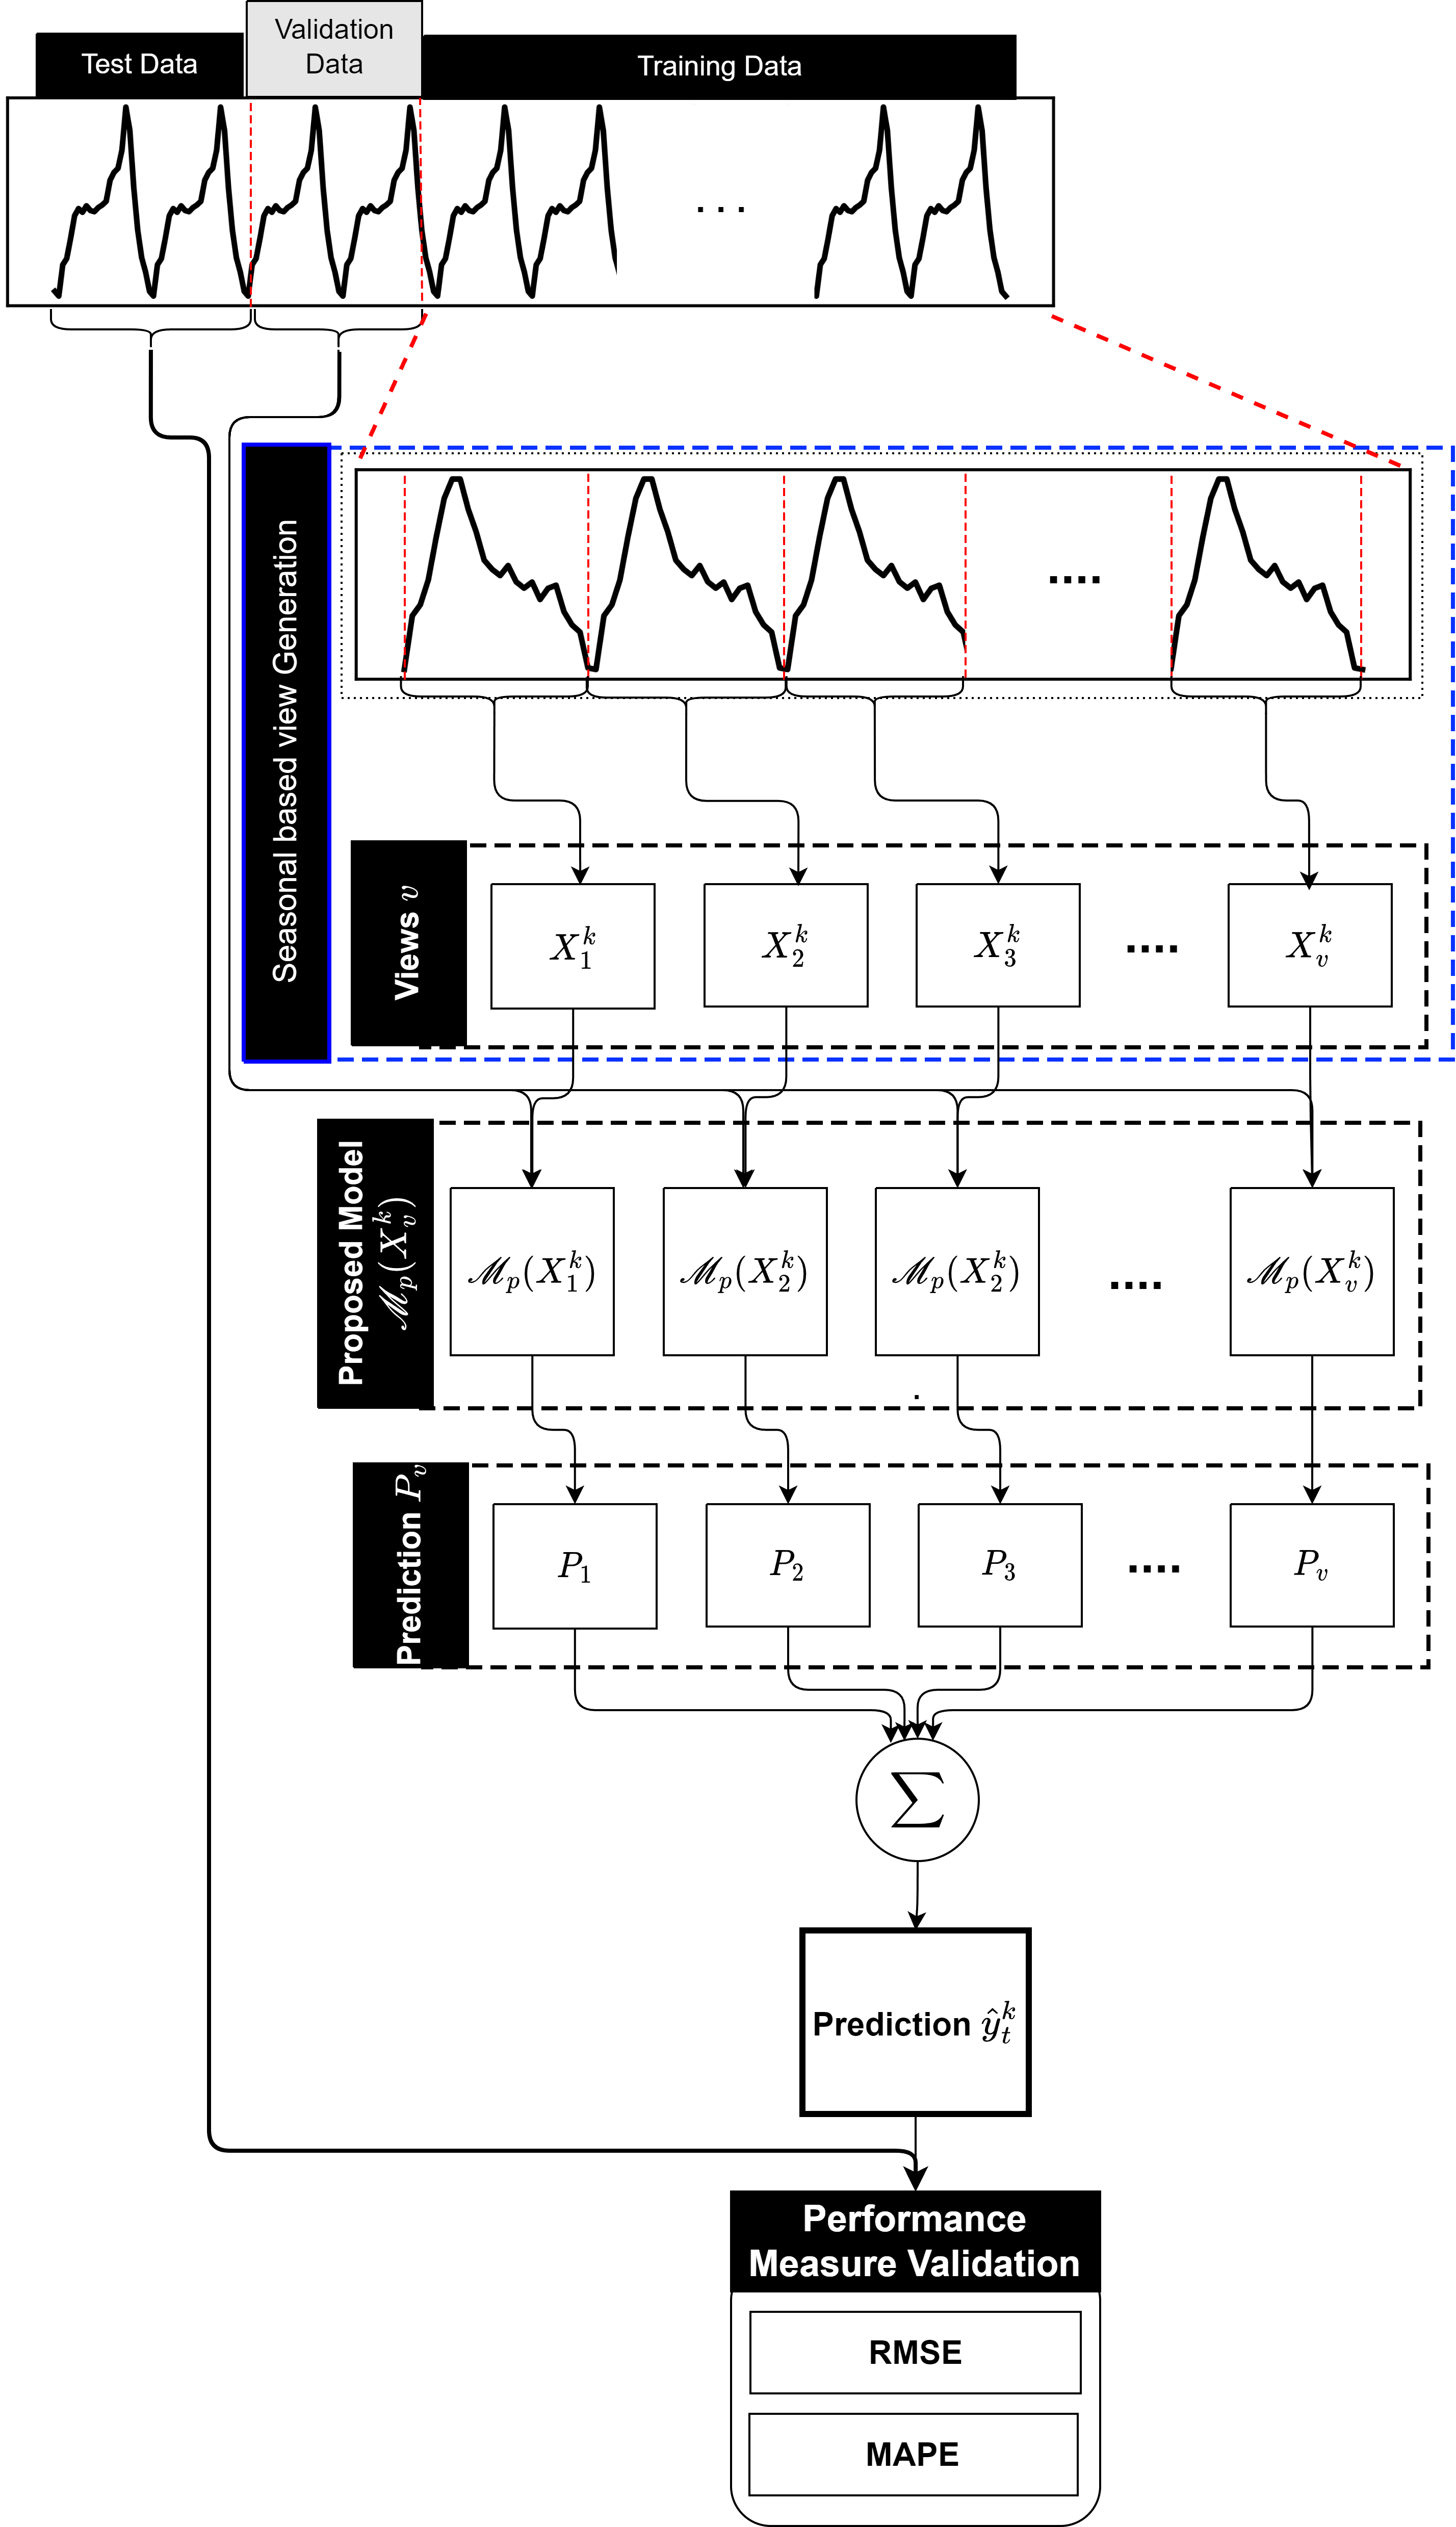
\includegraphics[scale=0.6]{MvS CNN-BiLSTM}
	  \caption{Flow diagram of proposed Multi-view Stacked CNN-BiLSTM (MvS CNN-BiLSTM)}\label{Muticbilstm}
\end{figure*}
\subsection{Model Devlopment}
Let's $X_v=[ x_1, x_2, x_3, \dots ,x_m]$ is a univariate time series (see the \Cref{univts}),  where $i^{th}$ data point $x_i \in X$,  $X \in \mathbb{R}^m$ and $m$ is the length of the time series which follow the ergodic properties (see the \Cref{ep uv}). It means time series X should not have the following: 

\begin{itemize}
  \item \textbf{High-variability : } The cowehy-distributed i.i.d $X $ has $\bar{x}\underset{d}{=} x_1$ which means,  high variability of marginal distribution function.
  \item \textbf{Lock of stability : } The $X$ distribution changes too much for marginal distribution functions such as variance approaches to infinity.
  \item \textbf{Absorbing state : } The range of probability measure varies from 0 to 1.
\end{itemize}
It is also assumed that the univariate time series X is at least weakly stationary or strictly stationary.


\begin{definition}[Univariate time series] \label{univts}
  "A univariate time series $X=[x_1, x_2, \dots, x_m]$,  $X\in \mathbb{R}^m$ is an orderd sequence of sigle dimensional vactor,  where $x_i$ denotes the $i^{th}$ time stamp observation and length of series is $m$."
\end{definition}

  \begin{definition}[Multi-view univariate time series]\label{mvts}
    "A multi-view univariate time series is a set of a subset $V^k= \{X_{v} \}_{v=1}^k$ of univariate time series $X\in \mathbb{R}^m$,  where ($k$ total number of view ) $v^{th}$ view from $X$ is observed as $X_v \subseteq X$ \& $X_v \in \mathbb{R}^{m_v}$,  $m_{v} < m$,  $\left|X  \right|= \sum_{v=1}^{K} \left| X_{(v)} \right|$ and view univariate series denoted as $X_v=[ x_t, x_{t+1}, x_{t+2}, \dots, x_{t+m_v} ]$ ."
  \end{definition} 

  \begin{definition}[$v^{th}$-Views of univariate time series]\label{v uts}
    "A $v^{th}$-view $X_v=[ x_t, x_{t+1}, x_{t+2}, \dots, x_{t+m_v} ]$ of univariate of time series $X$ is $X_v \subset X \in \mathbb{R}^{m}$ \& $X_v \in \mathbb{R}^{m_v}$ ,  where $m_{v} < m$,  and $m$ \& $m_v$ is the length of time series $X$ and $X_v$ . "
  \end{definition}

  \begin{definition}[Ergodic property of univariate time series]\label{ep uv}
    "A time series has the long-term time mean of a process is equivalent to the mean of all possible realisation of the time series."    
  \end{definition}

\begin{enumerate}[label=(\alph*)]

\item \textbf{Measuring strength of seasonality by decomposition of series $X$ :}\\
the decomposition of time series $X$ can be represented  as 

\begin{equation}
  \label{x}
  X = X^T + X^S +X^R
\end{equation}

where Trend component : $X^T$,  Seasonal component :  $X^S$ and Remainder component :  $X^R$ are denoted respectively. 
The strength of seasonality $F_S$ can be defined as \Cref{fs}: 

\begin{equation}\label{fs}
  F_S=max \left(0, 1- \frac{Var (X^R)}{Var(X^S + X^R)} \right)
\end{equation}

Where Var($V^R$) and Var($X^S + X^R$) are the variance of Remainder and detrended data over seasonal and Remainder, respectively and $F_S$ close to 0 and 1 exhibits no seasonality and strong seasonality.

\item \textbf{Identifying seasonal for lowest lag $\mathscr{L}$ :} \\
The coefficient of Auto Correlation Function (ACF) for lag $\mathscr{L}$ for time series $X$ can be obtained as in \Cref{rovh}: 

\begin{equation}
  \label{rovh}
  \rho_{\mathscr{L}}=\frac{E(x_t - \mu)(x_{t+ \mathscr{L}}-\mu)}{\sigma_x^2}
\end{equation}

where $\mu=E(X_t)$ is constant mean and $\sigma_x^2 = \frac{1}{m} \sum_{t=1}^{m} (X_t - \bar{X} )^2$,  $\bar{X}= \left(\frac{1}{m} \right) \sum_{t=1}^{m} X_t$ is the sample mean the coefficients $\rho_\mathscr{L}$ of auto correlation function has range $[-1,  +1]$,  where close to $+1$ exhibits the strong positive lag. Let's consider $\rho_\mathscr{L}^+$ is a set of ACF coefficients of lag that has a positive coefficient,  which can be denoted as

\begin{equation}\label{rhl}
  \rho_\mathscr{L}^+ ={\left\{ \rho_\mathscr{L} > 0 \right\}}_{\mathscr{L}=1}^{\left| \rho_{all}  \right|}
\end{equation} 

$\left|\rho_{all}  \right|$ :  Total no. of ACF coefficients.\\


Then the lowest lag value will indicate the smallest time stamp that has season behaviour in the series $X$, which can be identified as
\begin{equation} \label{lxl}
  \mathscr{L}_{lowest}^+ = \underset{\mathscr{L} \in \mathbb{R}}{arg min} \left\{\rho_{\mathscr{L}}^+  \right\}
\end{equation}



\item \textbf{Sesisonality based view generation($X_v^k \in X$ ) : } \\
Let's consider $T_{\mathscr{L} ^+}$ is the time stamp of the length of seasonal with lowest $\mathscr{L}_{lowest}^+$ lag; then the series $X$ can be partitioned with seasonal repetition for $\mathscr{L}^+$ lags,  where $k$- no. of partition can be obtained corresponding to $\mathscr{L}^+$. Figure \Cref{view gen} is the graphical representation of seasional of series $X$ corresponding to $\mathscr{L}_{lowest}^+$ lag.

The length of time stamp of $i^{th}$ partition $m_v$ (i.e. a view of $X$) can be obtained as \Cref{vvtk}.

\begin{equation} \label{vvtk}
  m_v=\frac{m}{T_{ \mathscr{L}_{lowest}^+ }\times k}
\end{equation}

where $m$ is the length of time stamp of $X$,  and $T_{ \mathscr{L}_{lowest}^+ }$ is the length of time stamp of lowest lag.
The total no. of possible partition ranges as $\left[1,  \frac{m}{T_{\mathscr{L}_{lowest}^+ }} \right]$
lets a view $X_v^k \in X$ denote as : 
\begin{equation} \label{vi g}
  X_v^k = [x_t, x_{t+1}, x_{t+2},  \dots , x_{t+m_v}]
\end{equation}

 for $k$- no. of partition with $m_v$ length of series,  is the $v^{th}$ view of the $k$- no. of view of $X$ (see the  \Cref{v uts}),  where $X=\cup_{v=1}^k {X_v^k}$ and $m= \sum_{v=1}^{k} m_v$, from \Cref{vvtk} (see the \Cref{mvts}).

 \begin{figure}\label{view gen}
  \centering
  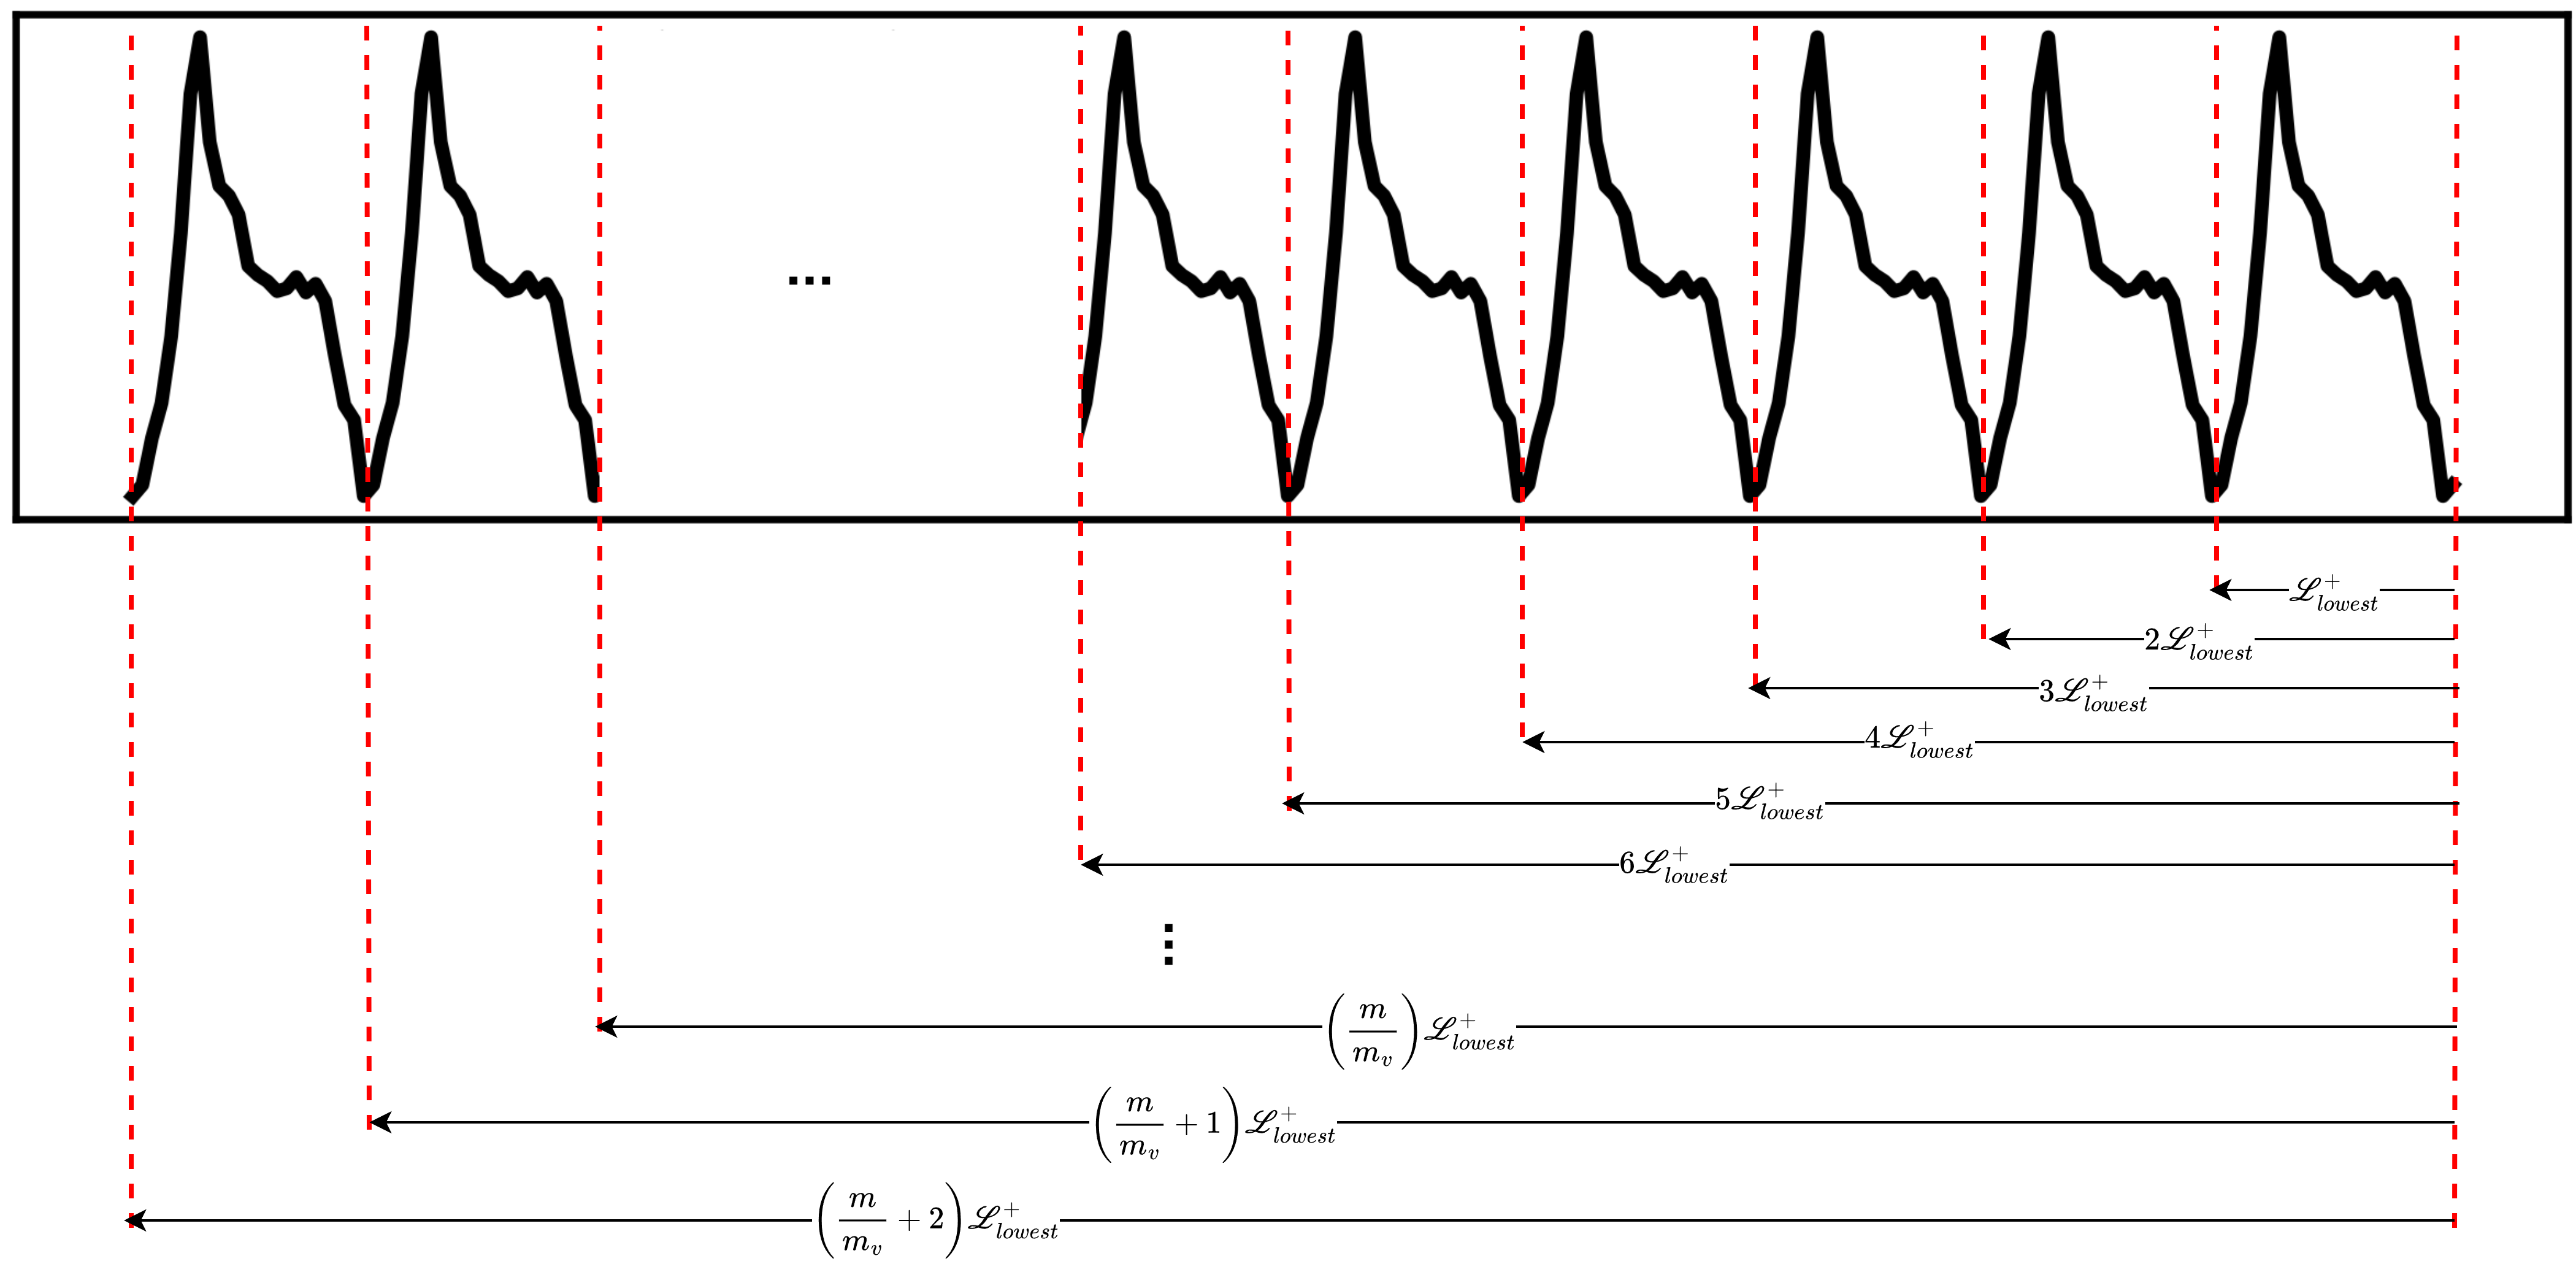
\includegraphics[scale=.6]{se_view}
  \caption{Sesisonality based view $X_v \in X$ generation.}
 \end{figure}


\item \textbf{Stacked CNN-BiLSTM : } \\
1D CNN layer for forward propagation is expressed as \Cref{1dcnn} : 
\begin{equation} \label{1dcnn}
  x_{(i, l)}^{(k, v)}=b_{(i, l)}^{(k, v)} + \sum_{j=1}^{L_{(l-1)}} conv1D \left(W_{(j, (l-1))}^{(k, v)},  S_{(j, (l-1))}^{(k, v)} \right)
\end{equation}
$L_{(l-1)}$ :  Number of neurons weight at $(l-1)$ layer.

$x_{(i, l)}^{(k, v)}$ :  $i^{th}$ input at $l$-layer of $v^{th}$ view $X_v^k$ for partion  $k$,  i.e.,  $x_{(i, l)}^{(k, v)} \in X_v^k$

$b_{(i, l)}^{(k, v)}$ :  defined as bias at $l$-layer.

$S_{(j, (l-1))}^{(k, v)}$ :  output of $j^{th}$ neurons at layer $(l-1)$.

$W_{(j, (l-1))}^{(k, v)}$ :  Kernal from the $j^{th}$ neuron at layer $(l-1)$.

$Conv1D (.)$ :  perform "in-valid" 1D convolution without zero padding.

And intermediate output $\hat{x}_{(i, l)}^{(k, v)}$ can be written as \Cref{1dd} :  
\begin{equation} \label{1dd}
  \hat{x}_{(i, l)}^{(k, v)}= f\left( x_{(i, l)}^{(k, v)} \right)
\end{equation}

In back-propagation,  the weight and bias are updated as follows : 
\begin{equation} \label{backp}
  W_{(i, (l-1))}^{(k, v)} (t+1) =W_{(i, l)}^{(k, v)}(t)- \varepsilon \frac{\partial E}{\partial W_{(i, (l-1))}^{(k, v)}}
\end{equation}

and 

\begin{equation} \label{bias}
  b_l^{(k, v)} (t+1) = b_l^{(k, v)}(t)- \varepsilon \frac{\partial E}{\partial b_l^{(k, v)}}
\end{equation}

where $\frac{\partial E}{\partial W_{(i, l-1)}^{(k, v)}} =conv1D \left(S_l^{(k, v)},  \Delta_{(l+1)}^{(k, v)} \right)$ and $\frac{\partial E}{\partial b_l^{(k, v)} }=\sum_{n}^{}\Delta_{l} (n)$. 
Then,  the find out come $\hat{x}_l^{(k, v)}$ of the 1DCNN may be written as \Cref{1dd hat}.

\begin{equation} \label{1dd hat}
  \hat{x}_l^{(k, v)}=\mathbb{F} \left(\hat{x}_{(i, l)}^{(k, v)} \right)
\end{equation}

where $\mathbb{F}(.)$ is activation function at last layer of the network. Now,  the input gate of BiLSTM can have $\hat{x}_i^{(k, v)}$ output of 1DCNN as input of BiLSTM shown in \Cref{si}.

\begin{equation}
\label{si}
  i_t^f = \sigma \left(W_{\left(\hat{x}_i^{(k, v)} \right)}^f  \cdot \hat{x}_i^{(k, v)} +W_{h_i}^f \cdot h_{(t-1)}^f +W_{c_i}^f \cdot c_{(t-1)}^f +b_i^f \right)
\end{equation}

Then, the final output gate can have output $\theta _{(t, 1)}^{(k, v)}$ for the fist stack

\begin{equation} \label{thi fin}
  \hat{y}_t^{(k, v)}=\theta _{(t, stack)}^{(k, v)}= \sigma \left(W_{\hat{x}_{out}^{(k, v)}} \cdot \hat{x}_{out}^{(k, v)} +  W_{h_{out}} \cdot h_t +W_{h_{out}} \cdot c_t +b_{out} \right)
\end{equation}

The stacked CNN-BiLSTM include repeating the same architecture shown from \Cref{1dcnn} to \Cref{thi fin}. Then the second stack output $\theta _{(t, 2)}^{(k, v)}$ can be obtained as \Cref{thi fin} which will corrosponding  to $v^{th}$ view of $x$ for $k$-partion. 



  \item \textbf{Multi-view Stacked CNN-BiLSTM Prediction : }\\
  The prediction of $v^{th}$ view $X_v \in X$ for $k$-partitioning is $\theta_{(t, 2)}^{(k, v)} $, so weighted ensemble of all view output for time $t$ is denoted as in \Cref{sta cb} .
  \begin{equation} \label{sta cb}
    \hat{y}_t^k= \left(\frac{1}{k} \right) \sum_{v=1}^{k} \left(\hat{y}_t^{(k, v)} \times \omega_v \right)
  \end{equation}
  where $\omega_v$ is the weight of view, i.e.,  the performance of stacked CNN-BiLSTM over validation set of $X$. over $v^{th}$ view $X_v$.



  \item \textbf{Finding best views of multi-view for learning of stacked CNN-BiLSTM : }\\
Let a set of final prediction of $k$-partition of X is denoted as  $\left\{\hat{y}_t^k \right\}_{k=\mathscr{L}_{lowest}^+}^{\mathscr{L}_{lowest}^+}$ and $\mathcal{M}_k(.)$ function to measure the performance of $k$-partition (for minimization). Then,  the best views $k_{best}$ can be exhibits as \Cref{bv}
  \begin{equation} \label{bv}
    k_{best}=\underset{t \in T}{arg min} \left\{\mathcal{M}_k \left(\hat{y}_t^k \right) \right\}_{k=\mathscr{L}_{lowest}^+}^{\mathscr{L}_{highest}^+}
  \end{equation}
  where $\mathscr{L}_{lowest}^+$ and $\mathscr{L}_{highest}^+$ are minimum and maximum of $\rho_{\mathscr{L}}^+$ ACF coefficient.

\end{enumerate}


\subsubsection{Proposed Multi-view Stacked CNN-BiLSTM (MvS CNN-BiLSTM)}
% Figure
\begin{figure*}[h!]
	\centering
		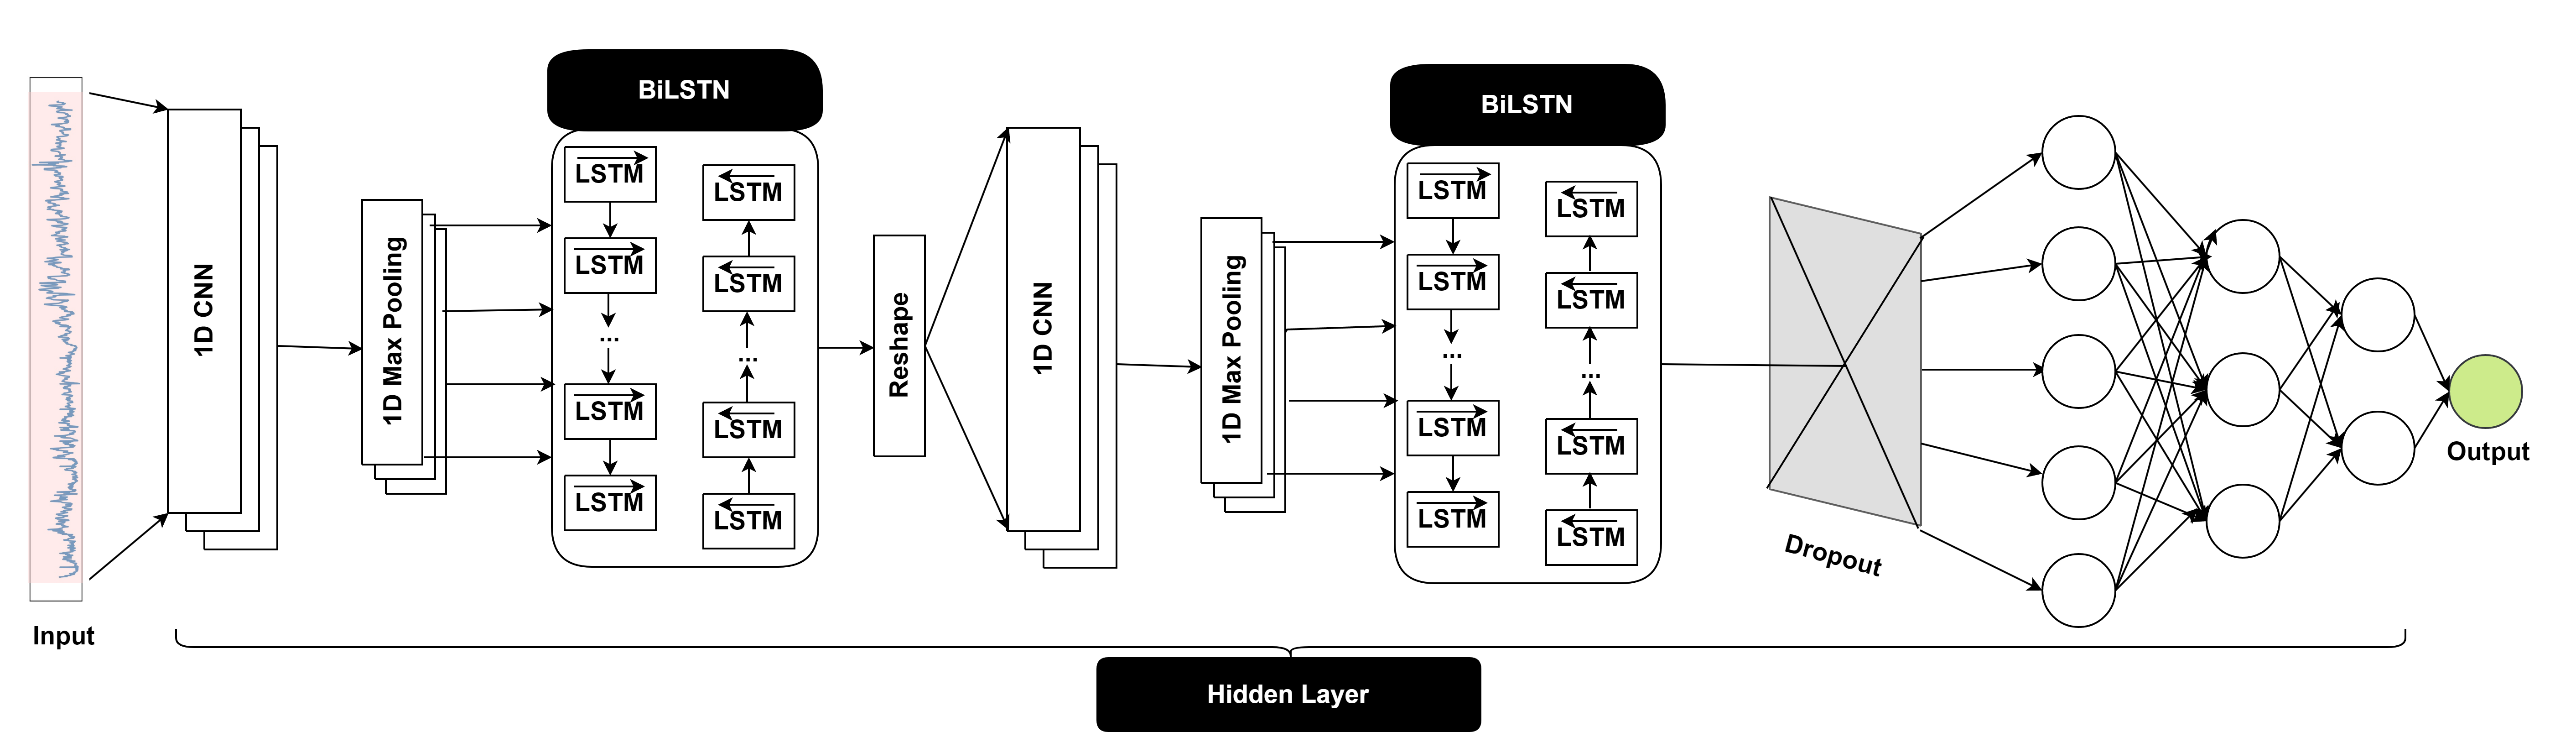
\includegraphics[scale=0.45]{Prpose}
	  \caption{Architecture of Stacked CNN-BiLSTM}\label{prosed_cnn-bilstm}
\end{figure*}

The model consists of various layers,  starting with a 1D Convolutional layer with 128 filters,  followed by a MaxPooling layer for downsampling. Next,  a Bidirectional LSTM layer with 64 units and ReLU activation is applied,  returning only the last output. A Reshape layer is introduced to reshape the output, and another 1D Convolutional layer with 32 filters is utilised,  followed by another MaxPooling layer. Another Bidirectional LSTM layer with 32 units and ReLU activation is added, returning only the last output. To prevent overfitting,  a Dropout layer with a rate of 0.2 is introduced before the final Dense layer,  which contains a single neuron for regression predictions. The model is given the name 'stacked CNN-BiLSTM'.

\subsubsection{Implamentation setup and parameters settings}
The various Python packages are utilised to implement the proposed and baseline models. These assortments incorporate Keras (v2.12.0),  TensorFlow (v2.12.0) for Keras backend, scikit-learn (v1.2.2) for model building and performance analysis,  Pandas (v1.5.3) \& NumPy (v1.23.5) for exploratory data analysis,  and matplotlib (v3.7.1),  seaborn (v0.12.2) \& Plotly (v5.14.1) for representing the results and plotting graphs.Additionally,  It have utilized \href{https: //app.diagrams.net/}{https: //app.diagrams.net/} for creating flowcharts. Two unique systems were employed for the experiments:  a Windows-based computer with an Intel\textregistered ~Core\texttrademark ~i7-11800H \texttt{@} 2.30GHz 8 GB RAM and a Kali Linux machine with an Intel\textregistered ~Core\texttrademark ~i7-4600U \texttt{@} 2.2GHz 16 GB RAM running JupyterLab (v4.0.1).


% \begin{table*}[h!]
%   \caption{Parameter setting of traditional DL models and proposed MvS CNN-BiLSTM }
%   \label{tab: my-table}
%   \begin{tabular}{ p{0.5\linewidth}  p{0.5\linewidth}}
%   \hline Hyperparameters & Values        \\ \hline
%   Batch Size               & 66                     \\
%   Optimizer                 & Adam                   \\
%   Loss function            & Mean Squared Error      \\
%   Epoch                    & 250 with early stopping \\
%   activation function      & ReLU                   \\
%   training size             & 0.8                   \\ \hline
%   \end{tabular}
%   \end{table*}



  \begin{table}[H]
    \setlength{\tabcolsep}{3pt}
    {\renewcommand{\arraystretch}{1}%
    \begin{longtable}[c]{ p{0.50\linewidth} p{0.50\linewidth} }
      \caption{Parameter setting of traditional DL models and proposed MvS CNN-BiLSTM}
      \label{tab: my-table}
    \\ \hline
    Hyperparameters & Values 
    \\ \hline
    \endhead
    %
    Batch Size               & 66                     \\
    Optimizer                 & Adam                   \\
    Loss function            & Mean Squared Error      \\
    Epoch                    & 250 with early stopping \\
    activation function      & ReLU                   \\
    training size             & 0.8                   \\ \hline
    \end{longtable}}
    \end{table}



\newcommand\mycommfont[1]{\footnotesize\ttfamily\textcolor{blue}{#1}}
\SetCommentSty{mycommfont}
\SetKwInput{KwInput}{Input}                % Set the Input
\SetKwInput{KwOutput}{Output}              % set the Output

\begin{algorithm}[!ht]
  \DontPrintSemicolon
  
    \KwInput{ $X=[x_1, x_2, x_3,  \dots , x_m] $,  where $x_i \in X$, $X \in \mathbb{R}^m$ and follows the ergodic properties.\\ $K \in \mathbb{N}^+$ \tcp*{no. of partition of series $X$ and ($v=1, 2, 3, 4 \dots$)} }
    \KwOutput{$X_v^k = [x_{(1, v)}, x_{(2, v)}, x_{(3, v)},  \dots , x_{(m_v, v)}]$,  where $x_i \in X_v^k$ \& $X_v^k \subset X$,  $m_v < m$  \tcp*{$v^{th}$ $k$- no. of partition of $X$ series.} }
    
  Initialization:  $k \in \mathbb{N}^+$\\ 
  indentfying seasional for lower lag $\mathscr{L}$ using ACF coefficient $\rho_{\mathscr{L}}$ :  
  $\rho_{\mathscr{L}}=\frac{E (x_t-\mu) (x_{t+\mu} -\mu)}{\sigma_x^2}$ \tcp*{see \Cref{rovh}}
  Finding set of positive coefficient of ACF $\rho_{\mathscr{L}^+}$ :  
  $\rho_{\mathscr{L}^+}= \left\{\rho_{\mathscr{L}} > 0 \right\}_{(\mathscr{L}=1)}^{ \left| \rho_{all} \right|}$ \tcp*{see \Cref{rhl}}
  obtaining the lowest lag $\mathscr{L}_{lowest}^+$ :  
  $ \mathscr{L}_{lowest}^+ = \underset{\mathscr{L} \in \mathbb{R}}{arg min} \left\{\rho_{\mathscr{L}}^+  \right\}$ \tcp*{see \Cref{lxl}}
  Generation of $v^{th}$ view $X_v^k \in X$ for $k$-partion :  
  $m_v=\frac{m}{T_{ \mathscr{L}_{lowest}^+ }\times k}$ \tcp*{see \Cref{vvtk}}
  $X_v^k = [x_{(1, v)}, x_{(2, v)}, x_{(3, v)},  \dots , x_{(m_v, v)}]$

  Return ($X_v^k$)\\
  End
  \caption{Generation of multiple views from univariate time series $X$.}\label{alg1}
  \end{algorithm}
  


  \begin{algorithm}[!ht]
    \DontPrintSemicolon
    
      \KwInput{ $X_v^k = [x_{(1, v)}, x_{(2, v)}, x_{(3, v)},  \dots , x_{(m_v, v)}]$ \tcp*{fron \Cref{alg1} }}
      \KwOutput{$\hat{y}_t^{(k, v)'}$ \tcp*{output  at second stack of CNN-BiLSTM}}
      
    Initialization:  stack = 1\\ 
    \If{stack $\le$ 2}{
      1DCNN layer for forward propagation:   
       $x_{(i, l)}^{(k, v)}=b_{(i, l)}^{(k, v)} + \sum_{j=1}^{L_{(l-1)}} conv1D \left(W_{(j, (l-1))}^{(k, v)},  S_{(j, (l-1))}^{(k, v)} \right)$ \tcp*{see \Cref{1dcnn}}
      outcome of 1DCNN from last layer using activation function $\mathbb{F}(.)$ :  
      $\hat{x}_l^{(k, v)}=\mathbb{F} \left(\hat{x}_{(i, l)}^{(k, v)} \right)$ \tcp*{see \Cref{1dd hat}}
      The output of the previous step-2 is the input of the BiLSTM input Gate (forward) :  
      $i_t^f = \sigma \left(W_{\left(\hat{x}_i^{(k, v)} \right)}^f  \cdot \hat{x}_i^{(k, v)} +W_{h_i}^f \cdot h_{(t-1)}^f +W_{c_i}^f \cdot c_{(t-1)}^f +b_i^f \right)$ \tcp*{see \Cref{si}}
      Then output of BiLSTM $\theta_{(t,  stack)}^{(k, v)}$ can be recived as :  
      $\theta _{(t, stack)}^{(k, v)}= \sigma \left(W_{\hat{x}_{out}^{(k, v)}} \cdot \hat{x}_{out}^{(k, v)} +  W_{h_{out}} \cdot h_t +W_{h_{out}} \cdot c_t +b_{out} \right)$ \\
      Repeat step-2 to 6 for stack=2; then the final output can be written as : 
      $\hat{y}_t^{(k, v)}=\theta _{(t, stack)}^{(k, v)}= \sigma \left(W_{\hat{x}_{out}^{(k, v)}} \cdot \hat{x}_{out}^{(k, v)} +  W_{h_{out}} \cdot h_t +W_{h_{out}} \cdot c_t +b_{out} \right)$  \tcp*{see \Cref{thi fin}}

    }
    Return ($\hat{y}_t^{(k, v)'}$)\\
    End
    \caption{Stacked CNN-BiLSTM Model.}\label{alg2}
    \end{algorithm}



  \begin{algorithm}[!h]
    \DontPrintSemicolon
      
      \KwInput{$X=[x_1, x_2, x_3,  \dots , x_m] $,  $x_i \in X$, $X \in \mathbb{R}^m$ \tcp*{Time series data (univariate).}, $K \in \mathbb{N}^+$ \tcp*{no. of partition of series $X$}.}
      \KwOutput{$\hat{y}_t^k$ \tcp*{Find weight aggregation of all output of model induced from views $X_v$}}
    Initialization:  $K \in \mathbb{N}^+$,  $\hat{y}_t^{(k, v)}= \left\{\phi \right\}$\\ 
    Checking ergodicity of univariate time series $X$ after preprocessing.\\
    Find the strength of seasonality of $X$ as $F_s$ : 
      $F_S=max \left(0, 1- \frac{Var (X^R)}{Var(X^S + X^R)} \right)$ \tcp*{see \Cref{fs}}
    \If{($F_s$ > 0)}{
      \For{$v=1$ to $k$ : }{
        Generating the $v^{th}$ view for $k$- partition from \Cref{alg1} i.e. $X_v^k$  \tcp*{\Cref{alg1}}
        Deployment of CNN-BiLSTM model \Cref{alg2} for the input series $X_v^k$,  then output recieved i.e. $\hat{y}_t^{(k, v)'}$ \tcp*{\Cref{alg2}} 
        Update the set of prediction of model induced with $v^{th}$ view $X_v^k$ as: 
        $\hat{y}_t^{(k, v)} \gets \left\{\hat{y}_t^{(k, v)}  \right\}  \cup \left\{\hat{y}_t^{(k, v)'}  \right\}$
      }
      Weighted aggregation of view-wise model prediction to get the find output $\hat{y}_t^k$ as: 
      $\hat{y}_t^k= \left(\frac{1}{k} \right) \sum_{v=1}^{k} \left(\hat{y}_t^{(k, v)} \times \omega_v \right)$ \tcp*{see \Cref{sta cb}}
    }
    Return ($\hat{y}_t^k$)\\
    End
    \caption{Stacked CNN-BiLSTM Model.}\label{alg3}
  \end{algorithm}



% \pagebreak


